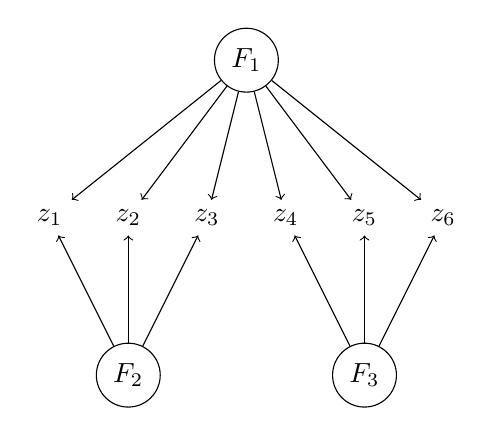
\begin{tikzpicture}
    \node[draw, circle] (F1) at (2.5,2) {$F_1$};
    \node[draw, circle] (F2) at (1,-2) {$F_2$};
    \node[draw, circle] (F3) at (4,-2) {$F_3$};

    \node (z1) at (0,0) {$z_1$};
    \node (z2) at (1,0) {$z_2$};
    \node (z3) at (2,0) {$z_3$};
    \node (z4) at (3,0) {$z_4$};
    \node (z5) at (4,0) {$z_5$};
    \node (z6) at (5,0) {$z_6$};

    \draw [->] (F1) edge (z1) (F1) edge (z2) (F1) edge (z3) 
               (F1) edge (z4) (F1) edge (z5) (F1) edge (z6);
    \draw [->] (F2) edge (z1) (F2) edge (z2) (F2) edge (z3);
    \draw [->] (F3) edge (z4) (F3) edge (z5) (F3) edge (z6);
\end{tikzpicture}

